\documentclass[11pt]{article}
\setlength{\textwidth}{6.3in}
\setlength{\textheight}{9in}
\setlength{\oddsidemargin}{0in}
\setlength{\evensidemargin}{0in}
\setlength{\topmargin}{-.6in}
\linespread{1.3}

% \renewcommand{\labelenumi}{\alph{enumi}}
\usepackage{epsfig}
\usepackage{amsmath}
\usepackage{bm}
\usepackage{amssymb}
\usepackage{amsfonts}
\usepackage{graphicx}
\newcommand{\spacer}{\displaystyle{\phantom{\int}}}
\newcommand{\blank}[1]{\underline{\hspace{#1}}}
\newcommand{\diff}[2]{\frac{d#1}{d#2}}
\newcommand{\difftwo}[2]{\frac{d^2#1}{d{#2}^2}}
\newcommand\dd[2]{\frac{\partial{#1}}{\partial{#2}}}
\newenvironment{piecewise}{\left\{\begin{array}{l@{,\quad}l}}{\end{array}\right.}
\newcommand{\col}[3]{\begin{bmatrix} #1 \\ #2 \\ #3 \end{bmatrix}}
\newcommand{\coll}[4]{\begin{bmatrix} #1 \\ #2 \\ #3 \\ #4\end{bmatrix}}
\DeclareMathOperator{\Span}{Span}
\DeclareMathOperator{\range}{range}
\DeclareMathOperator{\rank}{rank}
\DeclareMathOperator{\adj}{adj}
\newcommand{\points}[1]{({\it #1 points})}
\newcommand{\I}{\mathbb{I}}
\newcommand{\T}{\bm{\theta}}
\newcommand{\A}{\bm{\alpha}}
\def\dx{\Delta x}
\def\dsst{\displaystyle}
\hyphenation{}

% \epsfxsize=3.25in \epsfbox{line.eps}

\begin{document}
\noindent \textbf{Duke University  \hfill  November 2, 2016} \\
\noindent \textbf{CS 571D} \\
\line(1,0){455}
    
\begin{center}
\Large{{\bf HW 4}}\\
\end{center}

\begin{enumerate}

\item \begin{itemize}

\item Elements in our RKHS must be in the span of the $f(x_i)$'s. Thus, we start out with our RKHS equal to $H = \{ f(x) = \T^Tx\mid x \in \mathcal{X} \}$. \\ 

Now, we define a kernel in $H$ as follows: $k(x,z) = x^Tz$.

We see that this is just an inner product, so it clearly satisfies all the properties of inner products. \\ 

Now, let's show that $k$ is a reproducing kernel: 

\begin{align*}
\langle k(.,x),f \rangle = \T^Tx = f(x)\\
\end{align*}

Since we have defined $H$ and defined a reproducing kernel on $H$, we conclude that $H$ is a RKHS.

By the representer theorem, we know the optimal solution is in the form 
\begin{align*}
f^* = \sum_{i=1}^n \alpha_i x_i^T\cdot \\
\end{align*}
\item b 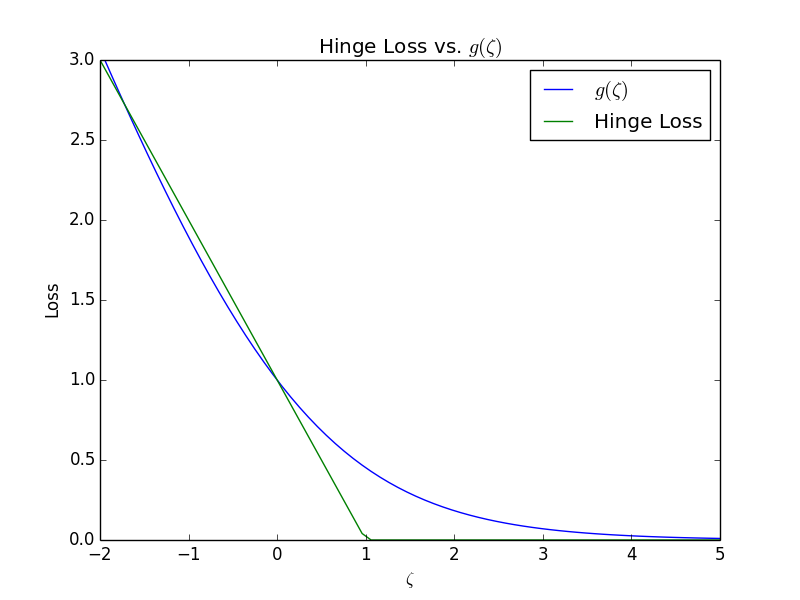
\includegraphics[scale=.75]{hinge_loss.png}
\item c: The $\ell_2$ regularized logistic regression problem can be written as the following primal problem:
\begin{align*}
& \text{min}_{\T,\theta_0,\zeta} \frac{1}{2}||\T||^2 + C \sum_{i=1}^ng(\zeta_i)\\
\end{align*}

subject to:
\begin{align*}
y_i(f(x_i) + \theta_0) \geq \zeta_i, \forall i
\end{align*}

This is equivalent to 
\begin{align*}\text{min}_{\T,\theta_0,\zeta} \frac{1}{2}||\T||^2 + C \sum_{i=1}^ng(\zeta_i) \; \; \text{s.t.} \; \; -y_i((f(x_i)+\theta_0) - \zeta_i) \leq 0 \forall i
\end{align*}

This leads to the Lagrangian
\begin{align*}
\mathcal{L}([\T,\theta_0],\A) = \frac{1}{2}\sum_{j=1}^n\theta_j^2 + C\sum_{i=1}^ng(\zeta_i) + \sum_{i=1}^n\alpha_i\left[-y_i(f(x_i)+\theta_0) - \zeta_i\right]
\end{align*}

We can write the KKT conditions, starting with Lagrangian stationarity.
\begin{align*}
&\nabla_{\T}\mathcal{L}([\T,\theta_0],\A) = \T - \sum_{i=1}^n \alpha_iy_i{\bf x}_i =0 \implies \T = \sum_{i=1}^n\alpha_iy_i{\bf x}_i\\
&\frac{d}{d\lambda_0}\mathcal{L}([\T,\theta_0],\A) = \sum_{i=1}^n\alpha_iy_i = 0 \implies \sum_{i=1}^n\alpha_iy_i = 0\\
&\forall i, \; \frac{d}{d \zeta_i} \mathcal{L} = \frac{Ce^{-\zeta_i}}{1+e^{-\zeta_i}} - \alpha_i = 0 \implies \zeta_i = \text{ln}(\frac{c}{a} - 1)\\
&\alpha_i \geq 0 \; \; \forall i  \; \; \text{(dual feasibility)}\\
&\alpha_i[-y_i(\T^Tx_i + \theta_0) + \zeta_i] = 0 \; \; \forall i  \; \; \text{(complementary slackness)}\\
&-y_i(\T^Tx_i + \theta_0) + \zeta_i \leq 0 \; \; \forall i  \; \; \text{(primal feasibility)}\\
\end{align*}
Using the KKT conditions, we can simplify the Lagrangian to get an expression for the dual:
\begin{align*}
\mathcal{L} &= \frac{1}{2}||\T||_2^2 + C\sum_{i=1}^ng(\zeta_i) + \T^T\sum_{i=1}^n(-\alpha_iy_ix_i) + \sum_{i=1}^n(-\alpha_iy_i\theta_0) + \sum_{i=1}^n\alpha_i\zeta_i\\
&= \frac{1}{2}||\T||^2 + C\sum_{i=1}^n\left[\ln \left( 1 + e^{-\zeta_i} \right) \right] + \sum_{i=1}^n\zeta_i\alpha_i\\
&= \frac{1}{2}||\T||^2 + C\sum_{i=1}^n\left[\ln \left( 1 + e^{-\ln\left(\frac{C}{\alpha_i} - 1\right)} \right) \right] + \sum_{i=1}^n\alpha_i \ln \left( \frac{C}{\alpha_i} -1 \right)\\
&= \frac{1}{2}||\T||^2 + C\sum_{i=1}^n\left[ \ln \frac{C}{\alpha_i} \right] + \sum_{i=1}^n\alpha_i \ln \left( \frac{C}{\alpha_i} -1 \right)\\
&= \frac{1}{2}||\T||^2 + nC \ln C+ \sum_{i=1}^n(\alpha_i - C) \ln (C - \alpha_i) - \sum_{i=1}^n\alpha_i \ln \alpha_i\\
\end{align*}

We can now formulate the dual problem:
\begin{align*}
\text{max}_{\bm{\alpha}} \mathcal{L}(\A)\\
\end{align*}
where
\begin{align*}
&\mathcal{L}(\A) = -\frac{1}{2}\sum_{i,k}\alpha_i\alpha_ky_iy_kx_i^Tx_k +  \sum_{i=1}^n(\alpha_i - C) \ln (C - \alpha_i) - \sum_{i=1}^n\alpha_i \ln \alpha_i\\
&\text{s.t.} \; \; \forall i \; \alpha_i \geq 0 \, \text{and} \,  0 \leq \alpha_i \leq C, \sum_{i=1}^n \alpha_iy_i = 0\\
\end{align*}
This is similar to the dual for the non-separable case of SVM in that the $\alpha$s are bounded by $C$ on top, but different in that there are more terms in the lagrangian. Specifically, there is an additional penalty for increasing the $\alpha$s, and the sum over the $\alpha$s has now been modified to involve a log and the C term.
\end{itemize}





\item a. Solving the optimization problem in SVM is equivalent to finding the maximum margin hyperplane, as shown in the notes. Therefore, if we can solve the SVM optimization problem for a data set of just two points, then two points are sufficient to find the maximum-margin hyperplane.\\

The SVM optimization problem with two points is the following:
\begin{align*}
\text{min}_{\bm{\lambda}, \lambda_0} \frac{1}{2} ||\bm{\lambda}||_2^2
\end{align*}
subject to:
\begin{align*}
\bm{\lambda}^Tx_1 + \lambda_0 + 1 \leq 0, - \bm{\lambda}^tx_2 - \lambda_0 + 1 \leq 0\\
\end{align*}

From here, we can form the lagrangian:
\begin{align*}
\mathcal{L}([\bm{\lambda},\lambda_0],\bm{\alpha}) = \frac{1}{2} \sum_{j=1}^p\lambda_j^2 + \alpha_1(\bm{\lambda}^tx_1 + \lambda_0 + 1) + \alpha_2(-\bm{\lambda}^Tx_2 - \lambda_0 + 1)
\end{align*}

We can take the gradient with respect to $\bm{\lambda}$:
\begin{align*}
\nabla_{\bm{\lambda}} \mathcal{L} = \bm{\lambda} + \alpha_1x_1 - \alpha_2x_2 =0 \implies \bm{\lambda} = \alpha_2x_2 - \alpha_2x_1
\end{align*}


We can take the derivative with respect to $\lambda_0$ and set it equal to zero, which implies that $\alpha_1 = \alpha_2$.

This also tells us that $\lambda_0 = 1- \bm{\lambda}x_1$.

We can take the gradient with respect to $\A$ and set it equal to zero, obtaining the equations $\alpha_1=\alpha_2=\frac{2}{||x_1-x_2||_2^2}$

Now, we have solved the problem. We have:

\begin{align*}
\bm{\lambda}&=\alpha_1y_1x_1 + \alpha_2y_2x_2\\
&=\frac{2}{||x_2-x_1||_2^2}(x_1 - x_1)\\
\lambda_0 &= \frac{||x_2||^2 - ||x_1||^2}{||x_1 - x_2||^2}
\end{align*}

	b. We call an optimization problem convex if it is in the form:
	\begin{align*}
	&\text{minimize} \; \; \; \;  \;f(x)\\
	&\text{subject to} \; \; \; \; g_i(x) \leq 0, i = 1, \dots, n\\
	\end{align*}
	and the functions $f(x), g_1(x), \dots, g_n(x)$ are all convex. In our case, $f = \frac{1}{2}||\lambda||_2^2$ and $g_i(x) = y_i(\lambda^Tx_i = \lambda_0) + 1 \leq 0$.
	We have that a function is convex if the Hessian $H$ of the function is positive semidefinite, where $H_{i,j} = \frac{d^2f}{dx_idx_j}$. This gives us a matrix that has 2 along the diagonals, and zero everywhere else. Let $d$ = dim($H$). Let $x \in \mathbb{R}^d$.
	\begin{align*}
	x^THx &=\\
	x^T2Ix &=\\
	2x^TIx &=\\
	2x^Tx &=\\
	2||x||^2 &\geq 0
	\end{align*}
	
Since $x^THx \geq 0 \forall x \in \mathbb{R}^d$, we H is positive semi-definite, and f is convex. Now, we just need to show that each $g_i$ is convex -- however, each $g_i$ is a line. Since all lines are convex, we have that the $g_i$ are convex, and therefore, the optimization problem is convex.

\item \begin{itemize}

\item a.

\item b. 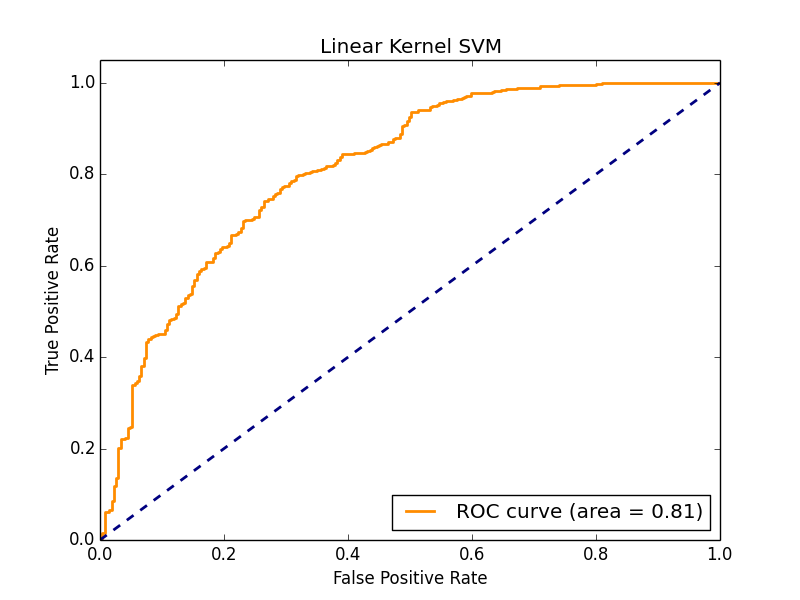
\includegraphics[scale=.75]{linear.png}\\

Accuracy: 0.839

\item c.  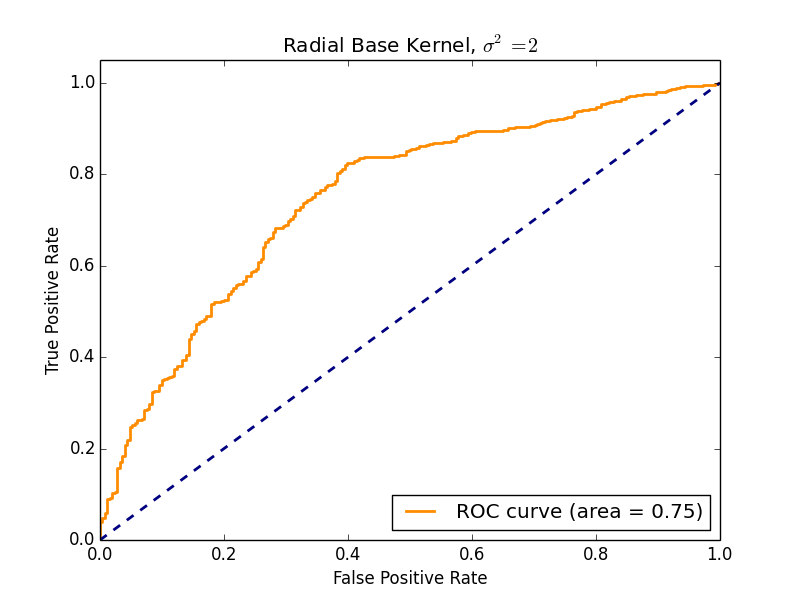
\includegraphics[scale=.75]{radial2.png}\\

Accuracy for $\sigma^2=2$: 0.785


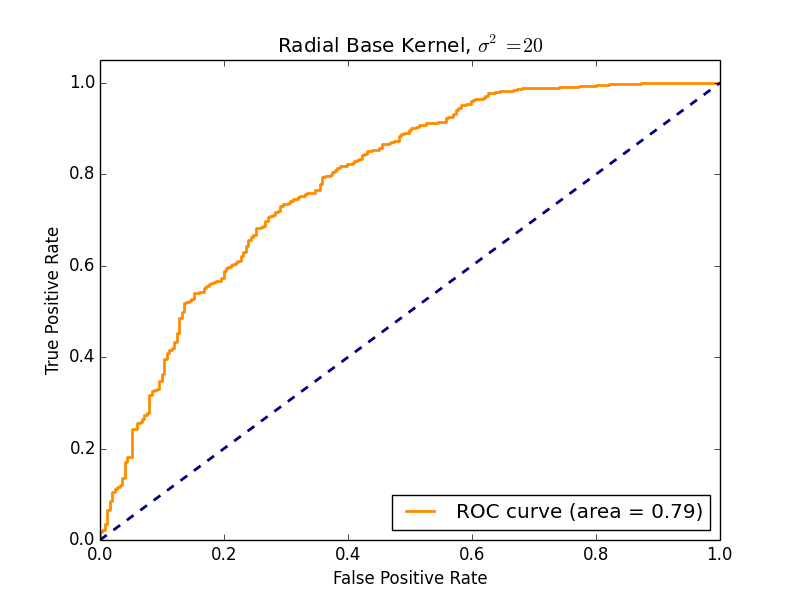
\includegraphics[scale=.75]{radial20.png}\\

Accuracy for $\sigma^2=20$: 0.836

\end{itemize}
\end{enumerate}



 
\end{document}
